\chapter{Dinámica efectiva}

En este capítulo se estudiarán, de una vez por todas, las dinámicas efectivas generadas por diferentes tipos de dinámicas microscópicas. Primero, motivados por el hecho de que el estado de máxima entropía es factorizable, se estudiará el caso de dinámicas generadas por Hamiltonianos que no tengan partes de interacción. Luego se analizarán compuertas de dos qubits bien conocidas en cómputo cuántico: la compuerta SWAP y la compuerta CNOT. Finalmente se profundizará en dinámicas más específicas, como un modelo de Ising uno-dimensional, así como evoluciones no unitarias, como el canal de despolarización, el canal de amortiguamiento de amplitud, entre otros.

\section{Dinámicas locales}

En la sección \ref{sec:Ch1PartialTrace} se habló de estados separables como aquellos estados que, descritos por un operador de densidad $\rho\in\densityspace{n}$, tienen la forma
\begin{equation}
    \rho=\rho_{A}\otimes\rho_{B},\nonumber
\end{equation}
donde $\rho_{A}\in\densityspace{m}$, $\rho_{B}\in\densityspace{l}$ y $l+m=n$. Siguiendo esta línea de pensamiento, con \textit{dinámicas factorizables} nos referimos a dinámicas unitarias generadas por hamiltonianos que no contienen un término de interacción (que en el caso de dos partículas son hamiltonianos de la forma $\mcH=H_{1}\otimes\Id+\Id\otimes H_{2}$), y que por lo mismo son descritas por operadores $\mcU\in\unitaryspace{n}$ del tipo
\begin{equation}
    \mcU=U_{A}\otimes U_{B}.\nonumber
\end{equation}
De nuevo, $U_{A}\in\unitaryspace{m}$, $U_{B}\in\unitaryspace{l}$ y $l+m=n$. Los operadores separables están compuestos por operadores que actúan de forma independiente sobre diferentes subsistemas del sistema en cuestión. En el caso de un sistema compuesto por dos subsistemas de dos niveles, el operador separable está compuesto por dos unitarias que actúan sobre $\hilbert_{2}$. Como el estado de máxima entropía resulta ser separable, las dinámicas separables son una muy buena primera forma de aplicar el formalismo descrito en las secciones anteriores.

Considérese la aplicación de grano grueso de $n$ a $1$ partículas definida según (\ref{eq:CG}), un estado efectivo $\rho_{\ef}\in\densityspace{2}$ y la aplicación de máxima entropía compatible dada por (\ref{eq:MaxEntAss}). Si la evolución microscópica es factorizable entonces es generada por un hamiltoniano de la forma
\begin{equation}
    \mcH=\sum_{k=1}^{n}\omega_{k}\Id_{2^{k-1}}\otimes H_{k} \otimes \Id_{2^{n-k}},\nonumber
\end{equation}
siendo la unitaria 
\begin{equation}\label{eq:NFactorUnitaries}
    \mcU_{t}=\Motimes_{k=1}^{n}\text{exp}\qty(-\rmi\omega_{k}H_{k}t)=\Motimes_{k=1}^{n} U_{k}(t).
\end{equation}
A partir de este momento, para hacer más limpia la lectura de este documento se omitirán los productos tensoriales con operadores identidad. El subsistema sobre el que actúe un operador será denotado por un subíndice, de tal manera que el hamiltoniano previamente definido queda
\begin{equation}
    \mcH=\sum_{k=1}^{n}\omega_{k}H_{k}.\nonumber
\end{equation}


\subsection{Caso general}

Si se considera una evolución unitaria de la forma (\ref{eq:NFactorUnitaries}), y se propaga al estado obtenido de la aplicación de máxima entropía, el estado evolucionado es
\begin{equation}
    \varrho_{\max}(t)=\Motimes_{k=1}^{n}\frac{1}{Z_{k}}U_{k}(t) e^{\qty(p_{k}\sum_{j}\lambda_{j}\pauli{j})} (U_{k}(t))^{\dag}\nonumber
\end{equation}
El estado efectivo evolucionado en términos de los multiplicadores de Lagrange queda
\begin{equation}\label{eq:SeparableEvolution}
    \Gamma_{t}(\rho_{\ef})=\sum_{k=1}^{n}p_{k} U_{k}(t) \rho_{k} (U_{k}(t))^{\dag}.
\end{equation}
donde $\rho_{k}=\frac{1}{Z_{k}}e^{\qty(p_{k}\sum_{j}\lambda_{j}\pauli{j})}$. 

Por supuesto, esta expresión puede expandirse en términos de exponenciales o de funciones hiperbólicas del vector de Bloch del estado efectivo inicial, $\vec{r}_{\ef}$. Haciendo esto se obtiene una expresión para el valor esperado de $\pauli{j}$ a un tiempo $t$,
\begin{equation}\label{eq:SeparableEvolutionExpVal}
    \expval{\pauli{i}(t)}=\frac{1}{2}\sum_{k=1}^{n}p_{k}\tanh(p_{k}\lambda)\Tr[\pauli{j}U_{k}(t) (\hat{r}_{\ef}\cdot\vec{\sigma}) (U_{k}(t))^{\dag}]
\end{equation}
Si se piensa en el caso en que $p_{1}>p_{j}\,\forall j\neq 1$, separar la contribución del sistema de interés,
\begin{align}
    \expval{\pauli{j}(t)}=&\frac{1}{2}p_{1}\tanh(p_{1}\lambda)\Tr[\pauli{j}U_{1}(t) (\hat{r}_{\ef}\cdot\vec{\sigma}) (U_{1}(t))^{\dag}]\nonumber\\
    &+\frac{1}{2}\sum_{k=2}^{n}p_{k}\tanh(p_{k}\lambda)\Tr[\pauli{j}U_{k}(t) (\hat{r}_{\ef}\cdot\vec{\sigma}) (U_{k}(t))^{\dag}]\nonumber,
\end{align}
permite reconocer dos términos: uno asociado a la evolución \textit{sin error} de nuestro sistema, descrita por el operador unitario $U_{1}(t)$, y un término de ruido. La acción de este término dependerá tanto de la naturaleza de las evoluciones locales del entorno, como del número de partículas en este.


Por otro lado, en el caso en el que no hay partícula prioritaria, \ie ($p_{j}=\frac{1}{n}\forall j$), la relación entre la magnitud del vector de Bloch del estado efectivo y los multiplicadores de Lagrange es $\lambda=n\tanh^{-1}(r)$. Esto significa que la expresión del valor esperado de $\sigma_{j}$ a un tiempo $t$ es
\begin{equation}
    \expval{\pauli{j}(t)}=\frac{1}{2n}\sum_{k=1}^{n}\Tr[\pauli{j}U_{k}(t) (\vec{r}_{\ef}\cdot\vec{\sigma}) (U_{k}(t))^{\dag}],\nonumber
\end{equation}
que no es más que una combinación lineal de las mismas componentes evolucionadas de formas diferentes.
\subsection{Ejemplos particulares}

\subsubsection{Dinámica simétrica}

Comenzamos con el caso en el que la dinámica separable simétrica, esto es, de una unitaria $\mcU\in\unitaryspace{2^{n}}$ de la forma
\begin{equation}
    \mcU_{t}=\Motimes_{k=1}^{n}U(t),\nonumber
\end{equation}
donde $U(t)\in\unitaryspace{2}$. Se aplica la evolución al estado de máxima entropía compatible con un conjunto de observables tomográficamente completos en $\hilbert_{2}$ y se propaga al estado con la unitaria subyacente, para luego pasarlo por la aplicación de grano grueso y recuperar el estado efectivo evolucionado. Este caso es quizá el más sencillo, pues la simetría de la unitaria permite factorizarla:
\begin{align}
\mcC\qty[\Motimes_{k=1}^{n}U(t) \rho_{k} (U(t))^{\dag}]&=\sum_{k=1}^{n}p_{k} U(t) \rho_{k} (U(t))^{\dag}\nonumber \\
&=U(t)\qty(\sum_{k=1}^{n}p_{k} \rho_{k}) (U(t))^{\dag}\nonumber\\
&=U(t)\rho_{\ef}(U(t))^{\dag}.\nonumber
\end{align}
La dinámica efectiva tiene la forma
\begin{equation}
    \Gamma_{t}(\rho_{\ef})=U(t)\rho_{\ef}(U(t))^{\dag}.\nonumber
\end{equation}
Este resultado es natural. No solo no hay interacción entre los diferentes subsistemas, significando esto que no se \textit{filtra} ningún tipo de información entre la partícula de interés y el resto, sino que cada parte evoluciona de manera idéntica: bajo la aplicación de grano grueso, lo que se observa es una combinación de $n$ entidades idénticas evolucionando de la misma forma.

\subsubsection{Particulas no preferenciales invariantes}

Centrémonos, momentáneamente, en el régimen $p_{1}>p_{j}\,\forall j\neq 1$. Asúmase que la probabilidad de detectar a la $k$-ésima partícula es la misma para todas excepto la primera. Entonces
\begin{equation}
    p_{k}=\frac{(1-p_{1})}{n-1}\text{ }\forall k\neq 1.\nonumber
\end{equation}
El estado de máxima entropía compatible con un estado efectivo $\rho_{\ef}$ es
\begin{equation}
    \varrho_{\max}=\rho_{1}\otimes\qty(\Motimes_{k=2}^{n}\frac{1}{Z_{k}}e^{\frac{(1-p_{1})}{n-1}\sum_{j}\lambda_{j}\pauli{j}}),\nonumber
\end{equation}
donde, para todo $k$ se cumple que
\begin{equation}
    \frac{1}{Z_{k}}e^{\frac{1-p_{1}}{n-1}\sum_{j}\lambda_{j}\pauli{j}}=\frac{1}{2}\qty(\Id+\tanh(\frac{1-p_{1}}{n-1}\lambda)\hat{r}_{\rho}\cdot\vec{\sigma})\equiv \rho_{\text{np}}.\nonumber
\end{equation}
El conjunto de partículas no preferenciales es entonces
\begin{equation}
    \Motimes_{k=2}^{n}\rho_{k}=\rho_{\text{np}}^{\otimes(n-1)}\nonumber.
\end{equation}
Si estas no varían, mientras que el subsistema de interés se propaga de forma unitaria, entonces la dinámica efectiva es
\begin{equation}
    \Gamma_{t}(\rho_{\ef})=p_{1}U(t)\rho_{1}(U(t))^{\dag}+(1-p_{1})\rho_{\text{np}}.\nonumber
\end{equation}
En términos del vector de Bloch del estado efectivo inicial, con $r_{1}=\tanh(p_{1}\lambda)$, $r_{\text{np}}=\tanh((1-p_{1})\lambda)$, y $R$ la rotación generada por $U$:
\begin{equation}
    r_{\ef}\hat{r}_{\ef}\mapsto p_{1}r_{1}R\hat{r}_{\ef}+(1-p_{1})r_{\text{np}}\hat{r}_{\ef}.\nonumber
\end{equation}
Esta expresión parece no dar demasiada información: es simplemente la combinación lineal de dos vectores de Bloch, uno que ha sido rotado y otro al que no se le ha hecho nada, pero recordando que el vector de Bloch del estado efectivo inicial cumple $r=p_{1}r_{1}+(1-p_{1})r_{\text{np}}$, esta puede ser manipulada para ver que
\begin{equation}
    r_{\ef}\hat{r}_{\ef}\mapsto R(r_{\ef}\hat{r}_{\ef}-(1-p_{1})r_{\text{np}}\hat{r}_{\ef})+(1-p_{1})r_{\text{np}}\hat{r}_{\ef}.\nonumber
\end{equation}
El resultado es una rotación alrededor de una línea que no pasa por el origen. Una rotación de esta naturaleza puede descomponerse en una rotación a través de un eje que pasa por el origen $R_{0}$ y una traslación $T$ como $T^{-1}\circ R_{0}\circ T$. Nótese que una transformación así no tendría por qué mantener a los estados dentro de la esfera de Bloch, por lo que esta debe depender del estado mismo. 

\begin{figure}[ht!]
    \centering
    \begin{subfigure}{0.32\textwidth}
      \centering
      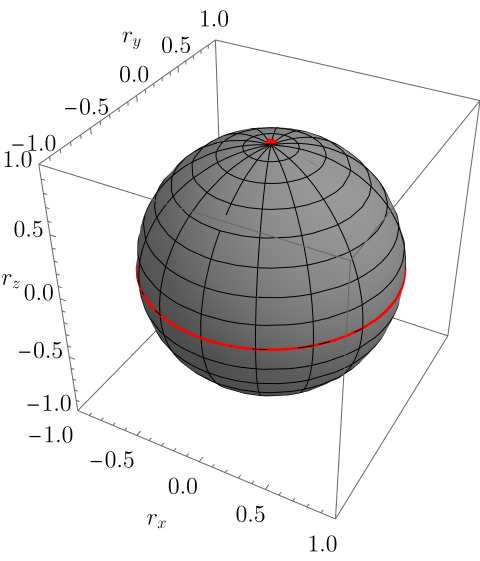
\includegraphics[width=0.9\linewidth]{chapter3/figures_separable/szxId_t=0._p=0.6_r=0.9.png}
      \caption{$t=0.0$}
    \end{subfigure}%
    \begin{subfigure}{0.32\textwidth}
      \centering
      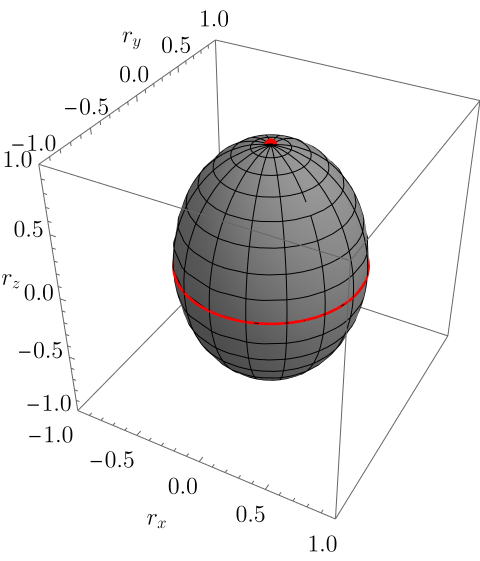
\includegraphics[width=0.9\linewidth]{chapter3/figures_separable/szxId_t=0.25_p=0.6_r=0.9.png}
      \caption{$t=0.25$}
    \end{subfigure}
    \begin{subfigure}{0.32\textwidth}
      \centering
      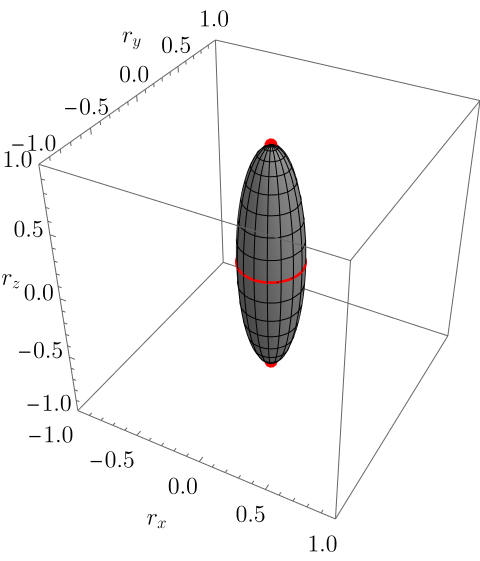
\includegraphics[width=0.9\linewidth]{chapter3/figures_separable/szxId_t=0.5_p=0.6_r=0.9.png}
      \caption{$t=0.5$}
    \end{subfigure}
    \caption{Efecto de la evolución subyacente sobre la esfera de Bloch si $r_{\ef}=0.9$, $p_{1}=0.6$ y $U=e^{-i\pi t \pauli{3}}$. La dramática contracción a lo largo de $z$ se asocia al alto valor de $1-p_{1}$.}
    \label{fig:FaseChangeSequence}
\end{figure}

En efecto, la traslación tiene una magnitud $(1-p_{1})r_{\text{np}}$ (a notar que la traslación es pequeña, y corresponde al término de ruido) en la dirección opuesta a la del estado (i.e. depende del estado tanto en magnitud como en dirección). Así que, aunque esto podría parecer una transformación afín, no lo es, pues depende enteramente del estado. Esto significa que la evolución efectiva no es lineal, y no tiene expresión en términos de operadores de Kraus. La figura \ref{fig:FaseChangeSequence} muestra el efecto que una dinámica de este estilo tiene sobre la esfera de Bloch (en particular, el caso $U_{1}=e^{-\rmi\omega t \pauli{3}}$). La contracción a lo largo del eje $z$ es un resultado del alto valor de $(1-p_{1})$ (0.4), y no sería visible si $p_{1}\rightarrow 1$.


En efecto, si $p_{1}\approx\frac{1}{2}$, entonces $\rho_{1}\approx\rho_{\text{np}}\approx\rho$ y la dinámica efectiva se convertiría en un canal de desfasamiento:

\begin{align}
    \Gamma_{t}(\rho_{\ef})=&p_{1}e^{-\rmi\omega t \pauli{3}}\rho_{1}e^{\rmi\omega t \pauli{3}}+(1-p_{1})\rho_{\text{np}}\nonumber\\
    \approx&\frac{1}{2}(\rho_{\ef}+e^{-\rmi\omega t \pauli{3}}\rho_{\ef} e^{\rmi\omega t \pauli{3}})\nonumber.
\end{align}

\subsubsection{Partícula preferencial invariante}

\acnote{Esta sección la tengo que volver a tocar}

Ahora asumamos que es el sistema preferencial el que no evoluciona, mientras que las demás partículas sí lo hacen. Existen diferentes formas de abordar este problema, según la elección de las probabilidades y de la naturaleza de la evolución del resto de las partículas. Quizá el caso más sencillo es aquel en el que todas las partículas no preferenciales evolucionan de la misma forma. Esto es, una evolución generada por un hamiltoniano de la forma
\begin{equation}
    \mcH=\omega \sum_{k=2}^{n}H_{k}.\nonumber
\end{equation}
Por simplicidad, tómese $H_{k}=\pauli{3}\,\forall k$. Recordando la ecuación (\ref{eq:rhoArhoB}), los valores de expectación de $\pauli{j}$ serán
\begin{align}
    \expval{\pauli{1}(t)}=&p_{1} \expval{\sigma_{1}(0)}_{1}+\sum_{k=2}^{n}p_{k}\Tr[\pauli{1}e^{-\rmi\omega t\pauli{3}} \rho_{k} e^{\rmi\omega t\pauli{3}}]\nonumber\\
    \expval{\pauli{2}(t)}=&p_{1} \expval{\sigma_{2}(0)}_{1}+\sum_{k=2}^{n}p_{k}\Tr[\pauli{2}e^{-\rmi\omega t\pauli{3}} \rho_{k} e^{\rmi\omega t\pauli{3}}]\nonumber\\
    \expval{\pauli{3}(t)}=&\expval{\pauli{3}(0)}_{\ef},\nonumber
\end{align}
que quizá sea más clara escribiéndose en términos de las componentes de los vectores de Bloch de cada partícula (el primer subíndice indica la componente del vector, mientras que el segundo denota la partícula a la que pertenece):
\begin{align}
    r_{1,\ef}(t)=&r_{1,1}(0)+\sum_{k=2}^{n}p_{k}(r_{1,k}\cos(2\omega t)-r_{2,k}\sin(2\omega t))\nonumber\\
    r_{2,\ef}(t)=&r_{2,1}(0)+\sum_{k=2}^{n}p_{k}(r_{2,k}\cos(2\omega t)+r_{1,k}\sin(2\omega t))\nonumber\\
    r_{3,\ef}(t)=&r_{3,\ef}(0).\nonumber
\end{align}
Esto no es más que la aplicación de la misma rotación sobre todos los vectores de Bloch, a excepción del primero. Reescribiendo,
\begin{align}
    \vec{r}_{\ef}(t)=&p_{1}\vec{r}_{1}+R_{z}(2\omega t)\vec{r}_{e}\nonumber\\
    =&\vec{r}_{\ef}(0)+(R_{z}(2\omega t)-\Id)\vec{r}_{e}\nonumber
\end{align}
donde $\vec{r}_{e}\sum_{k=2}^{n}p_{k}\vec{r}_{k}$.
En este caso, el primer término es el término invariante, y sería lo único visible en el caso en que el aparato de medición no fallara, mientras que el segundo término corresponde a pequeñas oscilaciones completamente dependientes del estado efectivo inicial que nunca aumentan la pureza del estado. En efecto, considérese un estado efectivo inicial correspondiente a un sistema microscópico de $10$ qubits cuyo vector de Bloch tiene radio $r_{\ef}=0.95$ y tal que $p_{1}=0.99$ y $p_{j}=\frac{0.01}{9}\,\forall\,j\neq $. La magnitud del error absoluto, esto es, la distancia del estado efectivo evolucionado al estado efectivo inicial es
\begin{equation}
    \mcO_{t}=\norm{\vec{r}_{\ef}(0)-p_{1}\vec{r}_{1}-R_{z}(2\omega t)\vec{r}_{e}}=\norm{\vec{r}_{e}-R_{z}(2\omega t)\vec{r}_{e}}\nonumber.
\end{equation}
Ahora, esta magnitud es máxima cuando $t=\frac{\pi}{2\omega}$, pero depende también de las componentes de $\vec{r}_{ef}$. Por simplicidad, asumamos que el estado efectivo inicial no tiene componente en $z$. Entonces
\begin{equation}
    \mcO_{\max}=\norm{-2\vec{r}_{e}}=1.08\times 10^{-3}\nonumber.
\end{equation}
Estas pequeñas oscilaciones son, justamente, el término de ruido. La visualización a la solución del problema puede observarse en la Figura \ref{fig:OscilationsSameHam}. Cada una de las componentes del vector de Bloch efectivo se ve como una suma de una constante con funciones periódicas que tienen el mismo periodo, o  como la suma de una constante más una función periódica (viendo la combinación de los vectores de cada partícula no preferencial como una partícula efectiva). De cualquier forma, el resultado es una función periódica.

\begin{figure}[ht!]
    \centering
    \begin{subfigure}{0.5\textwidth}
      \centering
      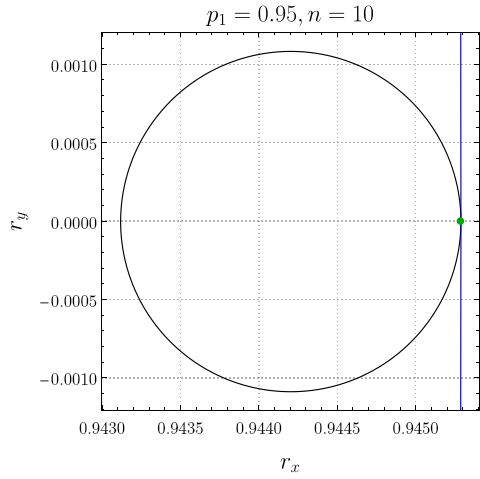
\includegraphics[width=0.9\linewidth]{chapter3/figures_separable/local_prefinv_eq_n=10_p=0.95.png}
      \caption{Nueve no preferencial}
    \end{subfigure}%
    \begin{subfigure}{0.5\textwidth}
      \centering
      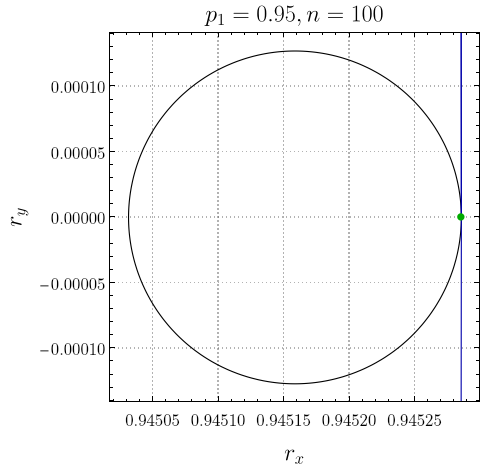
\includegraphics[width=0.9\linewidth]{chapter3/figures_separable/local_prefinv_eq_n=100_p=0.95.png}
      \caption{Noventa y nueve partículas no preferenciales}
    \end{subfigure}
    \caption{Oscilaciones periódicas cercanas al valor esperado. La periodicidad no depende de los pesos probabilísticos de cada partícula. En azul, el conjunto de estados con la misma pureza (y la misma coordenada en $\pauli{3}$) que el estado efectivo inicial (en verde).}\label{fig:OscilationsSameHam}
\end{figure}

Si, por otro lado, quitamos la restricción de que todas las partículas no preferenciales evolucionen con la misma frecuencia, se vuelve imposible factorizar la rotación:
\begin{equation}
    \vec{r}_{\ef}(t)=p_{1}\vec{r}_{1}+\sum_{k=2}^{n} p_{k}R_{z}(2\omega_{k} t)\vec{r}_{k}.\nonumber
\end{equation}
Ahora cada partícula no preferencial contribuye al error de forma única, y a pesar de que la evolución de cada partícula no preferencial sea periódica, la combinación de estas no tiene por qué serlo. El resultado ahora depende de las frecuencias de evolución de cada partícula, de sus pesos $p_{k}$, y del número $n$ de partículas en el sistema microscópico (si $n=2$ se recupera el caso anterior). Las componentes del vector de Bloch del estado efectivo evolucionado,
\begin{align}
    r_{1,\ef}(t)=&r_{1,1}(0)+\sum_{k=2}^{n}p_{k}(r_{1,k}\cos(2\omega_{k} t)-r_{2,k}\sin(2\omega_{k} t))\nonumber\\
    r_{2,\ef}(t)=&r_{2,1}(0)+\sum_{k=2}^{n}p_{k}(r_{2,k}\cos(2\omega_{k} t)+r_{1,k}\sin(2\omega_{k} t))\nonumber\\
    r_{3,\ef}(t)=&r_{3,\ef}(0).\nonumber
\end{align}
revelan la complejidad de la evolución, además de su no-linealidad, pues los vectores $\vec{r}_{k}$ dependen del estado efectivo inicial a través del multiplicador de Lagrange $\lambda.$ Las figuras \ref{fig:PrefInv1} y \ref{fig:PrefInv2} muestran algunos ejemplos de la geometría de estas dinámicas, en las que las frecuencias $\omega_{k}$ se obtuvieron de una distribución uniforme $\text{U}[-3,3]$.

\begin{figure}[ht!]
    \centering
    \begin{subfigure}{0.5\textwidth}
      \centering
      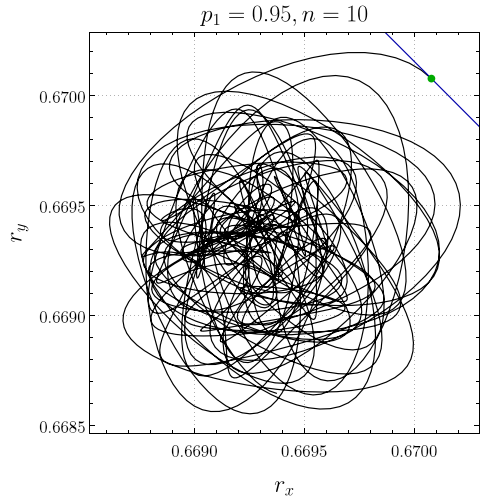
\includegraphics[width=0.9\linewidth]{chapter3/figures_separable/local_prefinv_ran_n=10_p=0.95_r=0.95_a=-3_b=3.png}
    \end{subfigure}%
    \begin{subfigure}{0.5\textwidth}
      \centering
      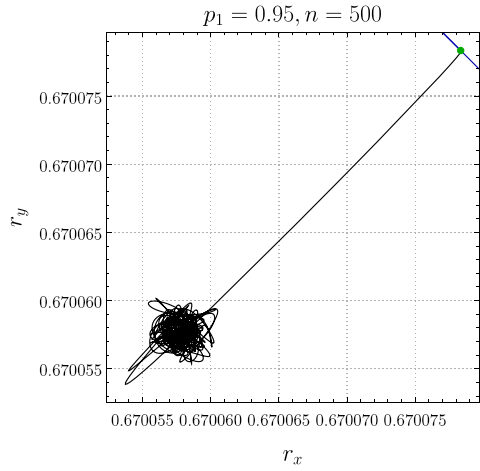
\includegraphics[width=0.9\linewidth]{chapter3/figures_separable/local_prefinv_ran_n=500_p=0.95_r=0.95_a=-3_b=3.png}
    \end{subfigure}
    \caption{Variaciones cercanas al estado efectivo inicial (verde). El aumento en el número de partículas lleva a una evolución complicada y no periódica, pero que converge al punto $\vec{r}_{1}$. En azul, el conjunto de estados con la misma pureza y la misma coordenada en $\pauli{3}$ que el estado efectivo inicial.}\label{fig:PrefInv1}
\end{figure}

\begin{figure}[ht!]
    \centering
    \begin{subfigure}{0.5\textwidth}
      \centering
      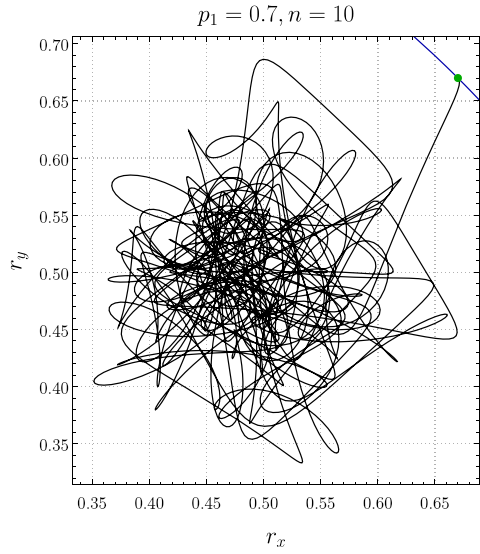
\includegraphics[width=0.9\linewidth]{chapter3/figures_separable/local_prefinv_ran_n=10_p=0.7_r=0.95_a=-3_b=3.png}
    \end{subfigure}%
    \begin{subfigure}{0.5\textwidth}
      \centering
      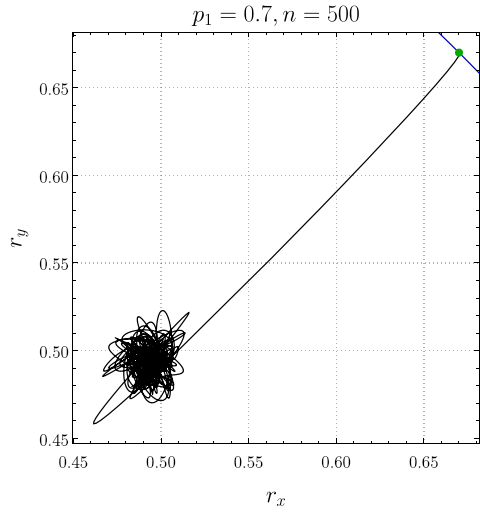
\includegraphics[width=0.9\linewidth]{chapter3/figures_separable/local_prefinv_ran_n=500_p=0.7_r=0.95_a=-3_b=3.png}
    \end{subfigure}
    \caption{Variaciones cercanas al estado efectivo inicial (verde). El aumento en el número de partículas lleva a una evolución complicada y no periódica, pero que converge al punto $\vec{r}_{1}$. Valores menos importantes de $p_{1}$ conducen a mayores variaciones. En azul, el conjunto de estados con la misma pureza y la misma coordenada en $\pauli{3}$ que el estado efectivo inicial.}\label{fig:PrefInv2}
\end{figure}

\subsubsection{Sistema en campo magnético ?}

\acnote{No tengo idea de qué justificación se pueda dar a que todas las partículas oscilen en la misma dirección pero con frecuencias diferentes.}

En los dos casos anteriores se permitió que alguna de las partes del sistema se mantuviera invariante, fuera la partícula preferencial o el resto. Veamos ahora qué sucede cuando se permite que todo el sistema evolucione. Considérese un hamiltoniano
\begin{equation}
    \mcH=\sum_{k=1}^{n}\omega_{k}\pauli{3,k},\nonumber
\end{equation}
de tal forma que toda la evolución mantenga constante la componente en $\pauli{3}$. Explícitamente, las componentes del vector de Bloch del estado efectivo siguen las ecuaciones
\begin{align}
    r_{1,\ef}(t)=&r_{1,1}(t)-\sum_{k=2}^{n}p_{k}A_{k}\sin(2\omega_{k} t-\phi_{k})\nonumber\\
    r_{2,\ef}(t)=&r_{2,1}(t)+\sum_{k=2}^{n}p_{k}A_{k}\sin(2\omega_{k} t+\theta_{k}),\nonumber
\end{align}
donde se omite la tercera componente, que no cambia, y
\begin{align}
    A_{k}=\sqrt{r_{1,k}^{2}+r_{2,k}^{2}} & & \phi=_{k}\arccos\qty(\frac{r_{2,k}}{\sqrt{r_{1,k}^{2}+r_{2,k}^{2}}}) & & \theta_{k}=\arcsin\qty(\frac{r_{1,k}}{\sqrt{r_{1,k}^{2}+r_{2,k}^{2}}})\nonumber
\end{align}
El comportamiento de los términos de suma depende de las frecuencias $\omega_{k}$, pero la amplitud de estas funciones oscilatorias puede acercarse arbitrariamente a $\sum_{k=2}^{n} p_{k} A_{k}$. Esto no significa que el error explote. En realidad, como $0\leq A_{k}\leq 1\,\forall k$, entonces $0\leq\sum_{k=2}^{n} p_{k} A_{k}\leq 1$. 


Para obtener resultados más específicos, asumamos que $p_{j}=p_{\text{np}}=\frac{1-p_{1}}{1-n}\,\forall\,j\neq 1$ y que $r_{3,\ef}=0$. Por construcción del estado de máxima entropía compatible con $\rho_{\ef}$,
\begin{align}
    r_{k}=r_{\text{np}}=\tanh(p_{\text{np}} \lambda) & & r_{j,k}=r_{\text{np}}\frac{r_{j,\ef}}{r_{\ef}}\nonumber
\end{align}
Esto significa que las expresiones previas se simplifican considerablemente, en efecto, las primeras dos componentes del vector pasan a ser
\begin{align}
    r_{1,\ef}(t)&=r_{1,1}(t)-p_{\text{np}}r_{\text{np}}\sum_{k=2}^{n}\sin(2\omega_{k} t-\phi)\nonumber\\
    r_{2,\ef}(t)&=r_{2,1}(t)+p_{\text{np}}r_{\text{np}}\sum_{k=2}^{n}\sin(2\omega_{k} t+\theta)\nonumber
\end{align}
Aquí pasa a ser claro que la amplitud máxima de la oscilación de error de cada componente es $(1-p_{1})r_{\text{np}}$, que en el caso en que $r_{\ef}=0.9$, $p=0.95$ y $n=100$ es $4.79\times 10^{-5}$, pero si $p_{1}=0.5$ es $0.4$. Las figuras \ref{fig:Oscilations12} y \ref{fig:Oscilations13} muestran algunos ejemplos de este tipo de dinámica.

\begin{figure}[ht!]
    \centering
    \begin{subfigure}{0.5\textwidth}
      \centering
      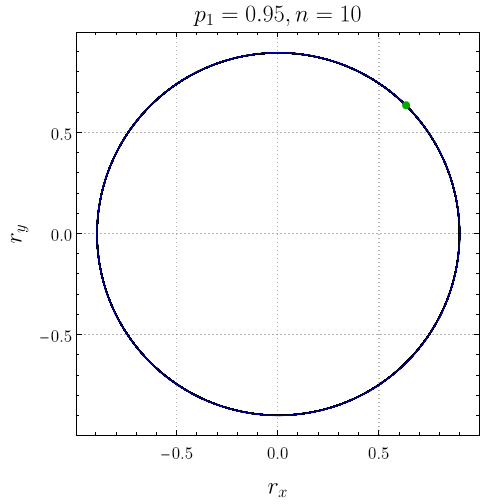
\includegraphics[width=0.9\linewidth]{chapter3/figures_separable/local_all_ran_p=0.95_r=0.9_n=10_a=-3_b=3.png}
    \end{subfigure}%
    \begin{subfigure}{0.5\textwidth}
      \centering
      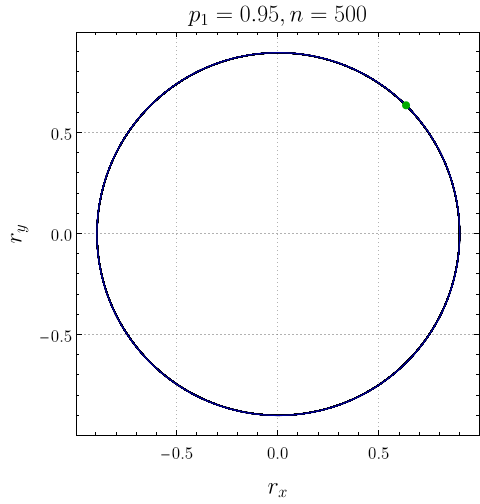
\includegraphics[width=0.9\linewidth]{chapter3/figures_separable/local_all_ran_p=0.95_r=0.9_n=500_a=-3_b=3.png}
    \end{subfigure}
    \caption{Como mencionado, para el caso en que $r_{\ef}=0.9$ y $p=0.95$ las variaciones debidas al error no son perceptibles debido a su pequeña amplitud, independientemente del número de partículas consideradas.}\label{fig:Oscilations12}
\end{figure}
\begin{figure}[ht!]
    \centering
    \begin{subfigure}{0.5\textwidth}
      \centering
      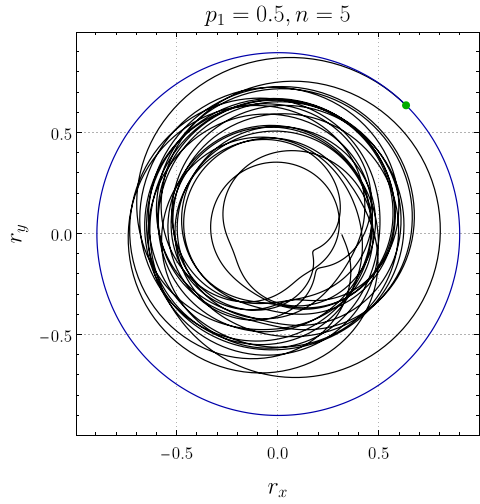
\includegraphics[width=0.9\linewidth]{chapter3/figures_separable/local_all_ran_p=0.5_r=0.9_n=5_a=-3_b=3.png}
    \end{subfigure}%
    \begin{subfigure}{0.5\textwidth}
      \centering
      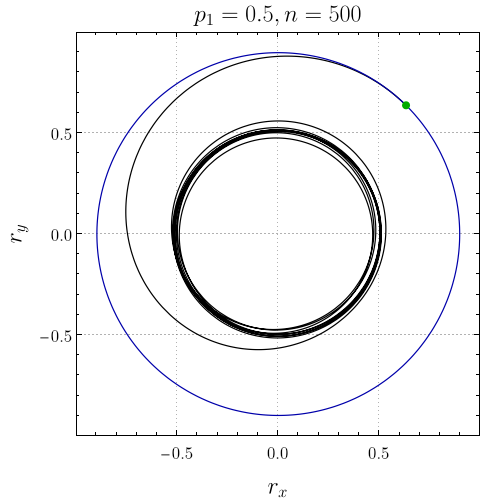
\includegraphics[width=0.9\linewidth]{chapter3/figures_separable/local_all_ran_p=0.5_r=0.9_n=500_a=-3_b=3.png}
    \end{subfigure}
    \caption{Si $r_{\ef}=0.9$ y $p=0.3$, el alejamiento de la evolución esperada se hace notar. Para valores grandes de $n$ se vuelve dominante el término de $p_{1}$}\label{fig:Oscilations13}
\end{figure}

\newpage

\pagebreak
\section{Construcción de la dinámica}
\notaAd{USAR MAPSTO EN LUGAR DE XRIGHTARROW}
\subsection{La compuerta cuántica SWAP}

\subsubsection{Acción de la compuerta}
La compuerta SWAP, $S$, actúa sobre dos qubits y los \textit{voltea}. Su acción sobre la base de $\hilbert_{4}$ contruida mediante los eigenestados de $\sigma_{3}\otimes\sigma_{3}$ es
\begin{align*}
    \ket{0}\otimes\ket{0}\xrightarrow{S}\ket{0}\otimes\ket{0}\\
    \ket{0}\otimes\ket{1}\xrightarrow{S}\ket{1}\otimes\ket{0}\\
    \ket{1}\otimes\ket{0}\xrightarrow{S}\ket{0}\otimes\ket{1}\\
    \ket{1}\otimes\ket{1}\xrightarrow{S}\ket{1}\otimes\ket{0} \rlap{.}
\end{align*}
Si un sistema está descrito por un operador de densidad separable, $\varrho=\rho_{A}\otimes\rho_{B}$, entonces el efecto de la compuerta SWAP es 
\begin{equation*}
    S\varrho S^{\dag}=\rho_{B}\otimes\rho_{A}.
\end{equation*}
La compuerta puede representarse como una matriz de permutación
\begin{equation*}
    S=\begin{pmatrix}
        1&0&0&0\\
        0&0&1&0\\
        0&1&0&0\\
        0&0&0&1
    \end{pmatrix}
\end{equation*}
\subsubsection{SWAP completo efectivo}

Utilizando la expresión (\ref{eq:MaxEntSeparable}), se puede pasar tanto a $\varrho_{max}(0)$ como a $\varrho_{max}(1)$ a través de la aplicación de grano grueso. El resultado $\CG{\varrho_{max}(0)}$ corresponde al estado grueso inicial, pero en términos de $\lambda$. Así:
\begin{equation}
\rho(0)=\frac{1}{2}[\Id+(\hat{r}_{\rho}\cdot\vec{\sigma})(p\tanh{-\lambda p}+(1-p)\tanh{-\lambda (1-p)})],
\end{equation}
\begin{equation}
\rho(t=1)=\frac{1}{2}[\Id+(\hat{r}_{\rho}\cdot\vec{\sigma})((1-p)\tanh{-\lambda p}+p\tanh{-\lambda (1-p)})].
\end{equation}
Vemos que ambos estados tienen la misma orientación pero pureza distinta. Esto significa que el efecto del \textsc{SWAP} subyacente sobre la esfera de Bloch es comprimir al estado efectivo inicial con un coeficiente $\kappa_{1}$ tal que
\begin{equation}\label{eq:SWAPFactor}
  \kappa_{1}=\frac{r_{\rho(1)}}{r_{\rho(0)}}=\frac{(1-p)\tanh{\lambda p}+p\tanh{\lambda (1-p)}}{
    p\tanh{\lambda p}+(1-p)\tanh{\lambda (1-p)}}
\end{equation}
Claro está, el factor de compresión depende del multiplicador de Lagrange, que a su vez es una función de la pureza del estado inicial. La figura \ref{fig:SWAPFactor2D} muestra dicha dependencia. Si la dependencia del factor de compresión en el estado efectivo inicial se denota por un superíndice, la dinámica efectiva puede escribirse como
\begin{equation}\label{eq:EffectiveSWAP1}
  \boxed{\frac{1}{2}(\Id+\vec{r}_{\rho}\cdot\vec{\sigma}) \xrightarrow{S} \frac{1}{2}(\Id+\kappa_{1}^{\rho}\vec{r}_{\rho}\cdot\vec{\sigma})}
\end{equation}
De las ecuaciónes (\ref{eq:SWAPFactor}) y (\ref{eq:EffectiveSWAP1}) distinguimos lo siguiente:
\begin{itemize}
  \item Si $p=0.5$, entonces $\kappa_{1}^{\rho}=1$. Esto se debe a que la aplicación borrosa es invariante bajo el $\textsc{SWAP}$ si $p=0.5$.
  \item $\kappa_{1}^{\rho}$ no depende de la orientación del vector de Bloch, únicamente depende de la magnitud $r_{\rho(0)}$ y $p$.
  \item En los casos extremos, $p=1$ o $p=0$, la esfera colapsa al origen.
\end{itemize}


Como el factor de compresión depende de $\lambda$, la dinámica no es lineal. Las operaciones cuánticas de un qubit se traducen como aplicaciones afines en la esfera de Bloch. Si quisiéramos ver el proceso asociado al \textsc{SWAP} subyacente como una transformación de la forma
\begin{equation*}
  \vec{r}\rightarrow M\vec{r}+\vec{c}
\end{equation*}
en la que $\vec{c}=0$, y $M=OS$ con $O=\Id$ y $S=\kappa_{1}(\vec{r})\Id$, de tal forma que
\begin{equation*}
  \vec{r}\rightarrow \kappa_{1}(\vec{r})\vec{r}
\end{equation*}
nos daríamos cuenta que la transformación no es afín, y por esto, el proceso no puede ser descrito a través del formalismo de las operaciones cuánticas (no tiene representación en operadores de Kraus) \cite{Chuang}.
\subsubsection{Caso $p=\frac{1}{2}$}

Aunque es posible repetir todas las cuentas desde la contrucción del estado de máxima entropía, haciendo $p=\frac{1}{2}$, basta con ver que el factor (\eqref{eq:SWAPFactor}) es $1$ en dicho caso. Así, todos los estado gruesos son puntos fijos bajo una evolución subyacente SWAP con aplicación de grano grueso con parámetro $p=\frac{1}{2}$.

\subsubsection{SWAP efectivo a un tiempo arbitrario}
Siendo \textsc{SWAP} un operador unitario, anteriormente se denotó el estado inicial y final como $\varrho(0)$ y $\varrho(1)$, de acuerdo a lo establecido en la ecuación (\ref{eq:TimeDepenenceUnitary}). Para extender los resultados a un tiempo arbitrario en el intervalo $[0,1]$, es necesaria una expresión analítica del operador. El operador SWAP deja intactos a los estados $\ket{00}$ y $\ket{11}$, e intercambia $\ket{01}$ con $\ket{1,0}$. De esto, el operador también dejará invariantes (hasta un factor) a los estados $\ket{+_{2}}=\frac{\ket{01}+\ket{10}}{\sqrt{2}}$ y $\ket{-_{2}}\frac{\ket{01}-\ket{10}}{\sqrt{2}}$. Dados estos eigenestados (y eigenvalores), la descomposición espectral del operador es
\begin{equation}\label{eq:SWAPSpectral}
S=P(\dyad{00}+\dyad{11}+\dyad{+_{2}}-\dyad{-_{2}})P^{\dag}.
\end{equation}
donde $P$ es la matriz formada por los eigenestados del operador. Potenciando se halla que
\begin{align}\label{eq:SWAPPower}
S^{t}&=P(\dyad{00}+\dyad{11}+\dyad{+_{2}}+(-)^{t}\dyad{-_{2}})P^{\dag}\\
&=P(\dyad{00}+\dyad{11}+\dyad{+_{2}}+e^{i \pi t}\dyad{-_{2}})P^{\dag}
\end{align}
La forma matricial del operador \textsc{SWAP} a un tiempo $t$ es
\begin{equation}
S^{t}=\begin{pmatrix}
 1 & 0 & 0 & 0 \\
 0 & \frac{1}{2}(1+e^{i \pi t}) & \frac{1}{2} (1-e^{i \pi t}) & 0 \\
 0 & \frac{1}{2}(1-e^{i \pi t}) & \frac{1}{2}(1+e^{i \pi t}) & 0 \\
 0 & 0 & 0 & 1
\end{pmatrix}=\begin{pmatrix}
  1 & 0 & 0 & 0 \\
  0 & e^{i\frac{t\pi}{2}}\cos{\frac{t\pi}{2}} & -ie^{i\frac{t\pi}{2}}\sin{\frac{t\pi}{2}} & 0 \\
  0 & -ie^{i\frac{t\pi}{2}}\sin{\frac{t\pi}{2}} & e^{i\frac{t\pi}{2}}\cos{\frac{t\pi}{2}}  & 0 \\
  0 & 0 & 0 & 1
 \end{pmatrix}
\end{equation}
Con ayuda de Mathematica pude aplicar este operador para obtener que
\begin{equation}
  \rho(t)=\frac{1}{2}\{\Id-(\hat{r_{\rho}}\cdot\vec{\sigma})[((1-p)\cos^{2}{\frac{\pi t}{2}}+p\sin^{2}{\frac{\pi t}{2}})\tanh{p\lambda}+(p\cos^{2}{\frac{\pi t}{2}}+(1-p)\sin^{2}{\frac{\pi t}{2}})\tanh{(1-p)\lambda}]\}.
\end{equation}
De esto, el factor de compresión dependiente del tiempo es
\begin{equation}\label{eq:SWAPFactort}
  \kappa_{t}^{\rho}=\frac{((1-p)\cos^{2}{\frac{\pi t}{2}}+p\sin^{2}{\frac{\pi t}{2}})\tanh{\lambda p}+(p\cos^{2}{\frac{\pi t}{2}}+(1-p)\sin^{2}{\frac{\pi t}{2}})\tanh{\lambda (1-p)}}{
    p\tanh{\lambda p}+(1-p)\tanh{\lambda (1-p)}}
\end{equation}
En términos del valor esperado del observable $\sigma_{z}$, la evolución del estado se da como
\begin{equation}
  \expval{\sigma_{z}(t)}=\kappa_{t}^{\rho}\cos{\alpha}
\end{equation}
que puede escribirse, también, como las probabilidades de que $\rho(t)$ se halle en el estado $\ket{0}$ o $\ket{1}$
 \begin{align}
  \bra{0}\rho(t)\ket{0}=\frac{1}{2}(1+\kappa_{t}^{\rho}\cos{\alpha}) && \bra{1}\rho(t)\ket{1}=\frac{1}{2}(1-\kappa_{t}^{\rho}\cos{\alpha})
 \end{align}
 donde la dependencia temporal está completamente contenida dentro del factor $\kappa_{t}^{\rho}$. 

\subsection{La compuerta cuántica CNOT}

\subsubsection{Acción de la compuerta}

La compuerta \textit{controlled not}, o CNOT, es el análogo cuántico de la compuerta lógica XOR \notaAd{CITA}. La compuerta XOR recibe como entrada dos bits, y arroja uno que puede ser $0$ si los bits de entrada tienen el mismo valor, o $1$ si tienen valores diferentes. Por otro lado, la compuerta cuántica CNOT actúa sobre un sistema de dos qubits, aplicando sobre el segundo qubit la compuerta $\sigma_{1}$ (NOT) si el primer qubit se halla en el estado $\ket{1}$, o dejándolo invariante si el primer qubit se halla en el estado $\ket{0}$. Esto es, cumple que \notaAd{CITA}
\begin{align*}
    \ket{0}\otimes\ket{0}\xrightarrow{\cnot}\ket{0}\otimes\ket{0}\\
    \ket{0}\otimes\ket{1}\xrightarrow{\cnot}\ket{0}\otimes\ket{1}\\
    \ket{1}\otimes\ket{0}\xrightarrow{\cnot}\ket{1}\otimes\ket{1}\\
    \ket{1}\otimes\ket{1}\xrightarrow{\cnot}\ket{1}\otimes\ket{0} \rlap{.}
\end{align*}
La compuerta puede representarse como una matriz de permutación
\begin{equation*}
    \cnot=\begin{pmatrix}
        1&0&0&0\\
        0&1&0&0\\
        0&0&0&1\\
        0&0&1&0
    \end{pmatrix}
\end{equation*}

\section{Dinámicas especiales}

\subsection{Canales de Pauli}

Los canales de Pauli son canales cuánticos en los que se aplica un operador de Pauli con alguna probabilidad. El canal de Pauli de un qubit más general está definido como
\begin{gather}
    P:\mcB(\hilbert_{2}) \rightarrow \mcB(\hilbert_{2})\nonumber\\
    P(\Delta)=\sum_{j=0}^{3}q_{j}\pauli{j}\Delta\pauli{j}\,\text{ con }\, \sum_{j=0}^{3}q_{j}=1\rlap{.}\nonumber
\end{gather}
Reconociendo que cualquiera de los tres operadores de Pauli puede escribirse en términos de los otros dos, se puede aprovechar la relación $-i\pauli{2}=\pauli{1}\pauli{3}$ para escribir a los canales de Pauli de una forma particularmente útil:
\begin{equation}
    P(\Delta)=\sum_{j,k=0}^{1}q_{j,k}\pauli{1}^{j}\pauli{3}^{k}\Delta\pauli{3}^{k}\pauli{1}^{j}.\nonumber
\end{equation}
A través de esta expresión se extienden los canales de Pauli de un qubit a $n$ qubits como \acnote{agregar cita}
\begin{gather}\label{eq:PauliChannelN}
    P:\mcB(\hilbert_{2^{n}}) \rightarrow \mcB(\hilbert_{2^{n}})\nonumber\\
    P(\Delta)=\sum_{\vec{j},\vec{k}}q_{\vec{j},\vec{k}}\pauli{1}^{\vec{j}}\pauli{3}^{\vec{k}}\Delta\pauli{3}^{\vec{k}}\pauli{1}^{\vec{j}}\rlap{.}
\end{gather}
donde $\pauli{j}^{\vec{k}}=\pauli{j}^{k_{1}}\otimes\pauli{j}^{k_{2}}\otimes ... \otimes \pauli{j}^{k_{n}}$ y las entradas $k_{l}$ del vector $\vec{k}$ solo pueden valer $0$ o $1$.

\subsubsection{Canales de desfasamiento}

Por canales de desfasamiento se entiende aquellos canales cuánticos cuyo efecto es amortiguar los elementos fuera de la diagonal del operador sobre el que actúan. A notar que esta definición es dependiente de la base sobre la que se está trabajando. Por ejemplo, sea $\rho\in\densityspace{2}$. Si se utiliza la base de eigenestados de $\pauli{3}$, entonces el canal
\begin{equation}
    \rho\mapsto q_{1}\rho + q_{2} \pauli{3}\rho\pauli{3}\nonumber
\end{equation}
es un canal de desfasamiento. En efecto, la acción de este canal sobre los elementos de matriz de $\rho$ es
\begin{equation}
    \begin{pmatrix}
        \rho_{0,0} & \rho_{0,1}\\
        \rho_{1,0} & \rho_{1,1}\\
    \end{pmatrix}\mapsto\begin{pmatrix}
        \rho_{0,0} & (q_{1}-q_{2})\rho_{0,1}\\
        (q_{1}-q_{2})\rho_{1,0} & \rho_{1,1}\\
    \end{pmatrix},\nonumber
\end{equation}
mientras que el canal de \textit{bit flip},
\begin{equation}
    \rho\mapsto q_{1}\rho + q_{2} \pauli{1}\rho\pauli{1},\nonumber
\end{equation}
no lo es, pues su acción sobre los elementos de matriz de $\rho$ es
\begin{equation}
    \begin{pmatrix}
        \rho_{0,0} & \rho_{0,1}\\
        \rho_{1,0} & \rho_{1,1}\\
    \end{pmatrix}\mapsto\begin{pmatrix}
        \frac{1}{2}\qty(1+(q_{1}-q_{2})(2\rho_{0,0}-1)) & \Re(\rho_{0,1})-\rmi(q_{1}-q_{2})\Im(\rho_{0,1})\\
        \Re(\rho_{1,0})+\rmi(q_{1}-q_{2})\Im(\rho_{1,0}) & \frac{1}{2}\qty(1-(q_{1}-q_{2})(1-2\rho_{1,1}))\\
    \end{pmatrix}.\nonumber
\end{equation}
Por supuesto, el canal de \textit{bit flip} es un canal de desfasamiento si se trabaja en la base de los eigenestados de $\pauli{1}$, pues en esta base, la acción del canal de \textit{bit flip} es
\begin{equation}
    \begin{pmatrix}
        \rho_{0,0} & \rho_{0,1}\\
        \rho_{1,0} & \rho_{1,1}\\
    \end{pmatrix}\mapsto\begin{pmatrix}
        \rho_{0,0} & (q_{1}-q_{2})\rho_{0,1}\\
        (q_{1}-q_{2})\rho_{1,0} & \rho_{1,1}\\
    \end{pmatrix}.\nonumber
\end{equation}
Para extender la noción de canal de desfasamiento a $n$ qubits, primero nótese que dada la base de $\hilbert_{2}$ conformada por los eigenestados de $\sigma{3}$, $\{\ket{e_{0}},\ket{e_{1}}\}$, es posible construir una base $\{e_{\vec{k}}\}_{\vec{k}}$ de $\hilbert_{2^{n}}$ como
\begin{equation}
    \{e_{\vec{k}}\}_{\vec{k}}=\left\{\ket{e_{\vec{k}}}\in\hilbert_{2^{n}}: \ket{e_{\vec{k}}}=\Motimes_{j=1}^{n}\ket{e_{k_{j}}},\,k_{j}\in\{0,1\}\right\} \rlap{.}\nonumber
\end{equation}
Esto es, tomando los productos tensoriales de los eigenestados de $\pauli{3}$ consigo mismos. De esta manera podemos estudiar dos canales de desfasamiento, el primero actuando en la base de productos tensoriales de eigenestados de $\pauli{3}$,
\begin{gather}
    P_{\pauli{3}}:\mcB(\hilbert_{2^{n}}) \rightarrow \mcB(\hilbert_{2^{n}})\nonumber\\
    P_{\pauli{3}}(\Delta)=\sum_{\vec{k}}q_{\vec{k}}\pauli{3}^{\vec{k}}\Delta\pauli{3}^{\vec{k}}\rlap{,}\nonumber
\end{gather}
que corresponde al canal de Pauli \ref{eq:PauliChannelN} cuando $\vec{j}=0$, y el segundo definido sobre la base de productos tensoriales de eigenestados de $\pauli{1}$,
\begin{gather}
    P_{\pauli{1}}:\mcB(\hilbert_{2^{n}}) \rightarrow \mcB(\hilbert_{2^{n}})\nonumber\\
    P_{\pauli{1}}(\Delta)=\sum_{\vec{j}}q_{\vec{j}}\pauli{1}^{\vec{j}}\Delta\pauli{1}^{\vec{j}}\rlap{,}\nonumber
\end{gather}
que corresponde al canal de Pauli \ref{eq:PauliChannelN} cuando $\vec{k}=0$. Es relativamente sencillo demostrar que si se escoge $q_{\vec{j}}=\frac{1-q_{\vec{0}}}{2^{n}-1}\,\forall\,\vec{j}\neq\vec{0}$, el efecto de estos canales es de reducir la amplitud de las componentes fuera de la diagonal en un factor de $(2q_{\vec{0}}-1)$. \acnote{Debe ser sencillo, el problema es que me hago bolas con los índices.}

Consideremos entonces en canal de desfasamiento de dos qubits en cualquiera de las dos direcciones discutidas y con probabilidades como mencionadas anteriormente. Sea $\rho_{\ef}$ un estado efectivo en $\densityspace{2}$ correspondiente a un sistema $\varrho \in \densityspace{2^{n}}$, y sea $\varrho_{\max}\in\densityspace{2^{n}}$ el estado de máxima entropía compatible con el estado efectivo. Si se propaga al estado de máxima entropía por medio de este canal y luego se pasa el resultado por la aplicación de grano grueso, el resultado es una dinámica efectiva
\begin{equation}
  \Gamma_{t}(\rho_{\ef})=\mcC\qty[\sum_{\vec{j}}q_{\vec{j}}\,\pauli{3}^{\vec{j}}\varrho_{\max}\pauli{3}^{\vec{j}}]=\mcC\qty[\sum_{\vec{j}}q_{\vec{j}}\,\qty(\Motimes_{k=1}^{n} \pauli{3}^{j_{k}}\rho_{k}\pauli{3}^{j_{k}})]\nonumber.\nonumber
\end{equation}
Para resolver el lado derecho de la ecuación, nótese que existen $2^{n}$ posibles vectores $\vec{j}$, y dentro de estos, $2^{n-1}$ tienen un $0$ o un $1$ en la $\nu$-ésima posición. Esto significa que hay $\frac{2^{n-1}}{n}$ ceros y $\frac{2^{n-1}}{n}$ unos en cada posible entrada de todos los $\vec{j}$. Entonces podemos usar el hecho de que tanto los operadores $\pauli{3}^{\vec{j}}$ como el estado de máxima entropía son factorizables, así como que la aplicación de grano es lineal para sumar sobre dichos ceros y unos:
\begin{align}
    \mcC\qty[\sum_{\vec{j}}q_{\vec{j}}\,\qty(\Motimes_{k=1}^{n} \pauli{3}^{j_{k}}\rho_{k}\pauli{3}^{j_{k}})]=&\sum_{\vec{j}}q_{\vec{j}}\sum_{k=1}^{n}p_{k}\pauli{3}^{j_{k}}\rho_{k}\pauli{3}^{j_{k}}\nonumber\\
    =&\sum_{\{j_{k}:j_{k}=0\}}q_{j_{k}}\sum_{k=1}^{n}p_{k}\pauli{3}^{j_{k}}\rho_{k}\pauli{3}^{j_{k}}+\sum_{\{j_{k}:j_{k}=1\}}q_{j_{k}}\sum_{k=1}^{n}p_{k}\pauli{3}^{j_{k}}\rho_{k}\pauli{3}^{j_{k}}\nonumber\\
    =&q_{\vec{0}}\qty(\sum_{k=1}^{n}p_{k}\rho_{k})+\frac{1-q_{\vec{0}}}{2^{n}-1}(2^{n-1}-1)\qty(\sum_{k=1}^{n}p_{k}\rho_{k})+\frac{1-q_{\vec{0}}}{2^{n}-1}2^{n-1}\qty(\sum_{k=1}^{n}\pauli{3}p_{k}\rho_{k}\pauli{3}).\nonumber
\end{align}
Con lo que la dinámica efectiva es
\begin{equation}
    \Gamma_{t}(\rho_{\ef})=\qty(q_{\vec{0}}+\frac{2^{n-1}-1}{2^{n}-1}(1-q_{\vec{0}}))\rho_{\ef}+\qty(\frac{2^{n-1}}{2^{n}-1}(1-q_{\vec{0}}))\pauli{3}\rho_{\ef}\pauli{3}.\nonumber
\end{equation}
Nótese que la dinámica efectiva es lineal, y que únicamente depende de del número de partículas en el sistema microscópico. Aún más, este es un canal de desfasamiento de un qubit en dirección de $\pauli{3}$. Este resultado es análogo para el canal $P_{\pauli{1}}$. Para recuperar un canal de desfasamiento total (en el que todos los elementos fuera de la diagonal se hacen cero) basta con elegir $q_{\vec{j}}=\frac{1}{2^{n}}\,\forall\,\vec{j}$. En dicho caso la dinámica efectiva se reduce a
\begin{equation}
    \Gamma_{t}(\rho_{\ef})=\frac{1}{2}(\rho_{\ef}+\pauli{3}\rho_{\ef}\pauli{3}).\nonumber
\end{equation}
Esto es, el desfasamiento total en $n$ partículas se traduce como un desfasamiento total en una partícula.


\subsubsection{Canal de despolarización}

El canal de despolarización es el canal cuántico que contrae de manera uniforme a todos los estados hacia el estado máximamente mezclado. Al canal de despolarización se le define como
\begin{gather}\label{eq:DepolarizingChannelN}
    D_{q}:\mcB(\hilbert_{2^{n}}) \rightarrow \mcB(\hilbert_{2^{n}})\nonumber\\
    D_{q}(\Delta)=q\Delta+(1-q)\Id_{2^{n}}\Tr(\Delta)\rlap{.}
\end{gather}
Ahora, nótese que el canal de despolarización total puede verse como una concatenación de dos canales de desfasamiento total, uno en dirección $\pauli{1}$ y luego otro en dirección $\pauli{3}$ (el orden es irrelevante). Para ver esto, es particularmente útil escribir a la matriz de densidad $\varrho\in\densityspace{2^{n}}$ en términos de las componentes de su vector de Bloch,
\begin{equation}
    \varrho=\frac{1}{2^{n}}\sum_{\vec{j},\vec{k}}\gamma_{\vec{j},\vec{k}}\pauli{1}^{\vec{j}}\pauli{3}^{\vec{k}},\nonumber
\end{equation}
y notar que el efecto de dichos canales se puede ver como
\begin{align}
  P_{\pauli{1}}(\varrho)=\frac{1}{2^{n}}\sum_{\vec{j},\vec{k}}\delta_{\vec{k},\vec{0}}\gamma_{\vec{j},\vec{k}}\pauli{1}^{\vec{j}}\pauli{3}^{\vec{k}}  & & \text{y} & & P_{\pauli{3}}(\varrho)=\frac{1}{2^{n}}\sum_{\vec{j},\vec{k}}\delta_{\vec{j},\vec{0}}\gamma_{\vec{j},\vec{k}}\pauli{1}^{\vec{j}}\pauli{3}^{\vec{k}} \nonumber
\end{align}
de tal forma que su composición es
\begin{align}
    \qty(P_{\pauli{1}}\circ P_{\pauli{3}})(\varrho)&=\frac{1}{2^{n}}\sum_{\vec{j},\vec{k}}\delta_{\vec{j},\vec{0}}\delta_{\vec{k},\vec{0}}\gamma_{\vec{j},\vec{k}}\pauli{1}^{\vec{j}}\pauli{3}^{\vec{k}}\nonumber\\
    &=\frac{1}{2^{n}}\gamma_{\vec{0},\vec{0}}\Id_{2^{n}}.\nonumber
\end{align}
Que es precisamente el efecto del canal de despolarización total. Ahora, sea $\rho_{\ef}$ un estado efectivo en $\densityspace{2}$ correspondiente a un sistema $\varrho \in \densityspace{2^{n}}$, y sea $\varrho_{\max}\in\densityspace{2^{n}}$ el estado de máxima entropía compatible con el estado efectivo. Es inmediato ver que la dinámica efectiva correspondiente a un canal de despolarización total es otro canal de despolarización total, i.e.
\begin{equation}
    \Gamma_{t}(\rho_{\ef})=\frac{1}{2}\Id_{2}.
\end{equation}
Ahora, sabiendo que
\begin{equation}
    \qty(P_{\pauli{1}}\circ P_{\pauli{3}})(\varrho)=\frac{1}{2^{2n}}\sum_{\vec{j},\vec{k}}\pauli{1}^{\vec{j}}\pauli{3}^{\vec{k}}\varrho\pauli{3}^{\vec{k}}\pauli{1}^{\vec{j}}=\frac{1}{2^{n}}\Id_{2^{n}}\nonumber
\end{equation}
la ecuación \ref{eq:DepolarizingChannelN} puede reescribirse como
\begin{equation}
    D_{q}(\varrho)=\frac{q(2^{2n}-1)+1}{2^{2n}}\varrho+\frac{(1-q)}{2^{2n}}\sum_{\vec{j}\land\vec{k}\neq\vec{0}}\pauli{1}^{\vec{j}}\pauli{3}^{\vec{k}}\varrho\pauli{3}^{\vec{k}}\pauli{1}^{\vec{j}}\nonumber
\end{equation}
Donde es explícitamente claro que el canal de despolarización es un canal de Pauli. La dinámica efectiva que corresponde al canal de despolarización no completo es simplemente
\begin{equation}
    \Gamma_{t}(\rho_{\ef})=q\rho_{\ef}+(1-q)\Id_{2}.\nonumber
\end{equation}
Esto es, la dinámica efectiva correspondiente a un canal de despolarización siempre es un canal de despolarización. Nótese que este resultado es muy similar al obtenido para una evolución unitaria subyacente generada por un Hamiltoniano de la forma $\mcH=H\otimes\Id+\Id\otimes H$. En dicho caso, la dinámica efectiva era, justamente, la unitaria generada por el Hamiltoniano $H$, esto como consecuencia de la simetría de la evolución: la misma para cada partícula, sin interacción. Este caso es el mismo, el canal de despolarización actúa de la misma forma sobre cada partícula, y es completamente isotrópico dentro del subespacio de cada partícula.

\subsection{Canal de estabilización}

El canal de amortiguamiento de amplitud funciona como un modelo simple de emisión espontánea. En efecto, un átomo de dos niveles acoplado a un campo electromagnético experimenta emisión espontánea, y puede demostrarse que este proceso corresponde a un canal de amortiguamiento de amplitud si se traza al campo y se considera que la frecuencia del campo es igual a la frecuencia de resonancia de transiciones entre los niveles del átomo. El canal de amortiguamiento de amplitud tiene el efecto de enviar todos los estados al estado base. Aquí estudiaremos un canal más sencillo, que envía todos los estados a un estado puro aleatorio $\ket{\psi}$ de forma exponencial en el tiempo, como si el átomo de dos niveles tendiera a estabilizarse en dicho estado.

Considérese entonces que un sistema de $n$ partículas evoluciona siguiendo el canal cuántico
\begin{gather}
    \mcE_{\psi,t}:\mcB(\hilbert_{2^{n}}) \rightarrow \mcB(\hilbert_{2^{n}})\nonumber\\
    \mcE_{\psi,t}(\Delta)=e^{-t\mu}\varrho+(1-e^{-t \mu})\dyad{\psi}\Tr(\Delta)\rlap{.}\nonumber
\end{gather}
donde $\dyad{\psi}\in \densityspace{2^{n}}$. Es importante señalar que si se escoge $n=1$ y $\ket{\psi}=\ket{0}$ no se recupera el canal de amortiguamiento de amplitud, pues el canal de amortiguamiento de amplitud tiene el siguiente efecto sobre la matriz de densidad
\begin{equation}
    \begin{pmatrix}
        \rho_{0,0} & \rho_{0,1} \\
        \rho_{1,0} & \rho_{1,1}
    \end{pmatrix}\mapsto\begin{pmatrix}
        (1-\gamma)\rho_{0,0}+\gamma & \sqrt{1-\gamma}\rho_{0,1} \\
        \sqrt{1-\gamma}\rho_{1,0} & (1-\gamma)\rho_{1,1}
    \end{pmatrix},\nonumber
\end{equation}
donde $\gamma$ puede verse como la probabilidad de emisión de un fotón, mientras que el canal $\mcE_{\ket{0},t}$ tiene el efecto
\begin{equation}
    \begin{pmatrix}
        \rho_{0,0} & \rho_{0,1} \\
        \rho_{1,0} & \rho_{1,1}
    \end{pmatrix}\mapsto\begin{pmatrix}
        (1-\gamma)\rho_{0,0}+\gamma & (1-\gamma)\rho_{0,1} \\
        (1-\gamma)\rho_{1,0} & (1-\gamma)\rho_{1,1}
    \end{pmatrix}.\nonumber
\end{equation}
donde se ha hecho $e^{\mu t}=\gamma$. Es claro que el canal de amortiguamiento y el canal de estabilización tienen efectos diferentes en las fases del estado. Aún más, mientras que la extensión del canal de estabilización a $n$ partículas es directa, la generalización del canal de amortiguamiento de amplitud es no trivial. \acnote{agregar cita.}

Ahora, sea $\rho_{\ef}$ un estado efectivo en $\densityspace{2}$ y $\varrho_{\max}$ el estado de máxima entropía en $\densityspace{2^{n}}$ compatible con este. Aplicando el modelo de grano grueso al estado de máxima entropía propagado por el canal de estabilización se obtiene que
\begin{equation}
    \Gamma_{t}(\rho_{\ef})=e^{-t\mu}\rho(0)+(1-e^{-t \mu})\mcC(\dyad{\psi}).\nonumber
\end{equation}
Obsérvese que la dinámica efectiva es un canal cuántico, pero no necesariamente un canal de estabilización, pues el estado al que tiende el sistema efectivo, $\mcC(\dyad{\psi})$ no tiene por qué ser un estado puro. En realidad, en el caso en que $\ket{\psi}$ es un estado máximamente entrelazado, $\mcC(\dyad{\psi})$ es el estado máximamente mezclado, de tal manera que la dinámica efectiva es un canal de despolarización.

\subsection{Cadena de espines de Heisenberg}

El modelo $XZY_{s}$ unodimensional de Heisenberg consiste en una cadena de $n$ partículas de espín $s$ en la que se consideran interacciones de espín entre primeros vecinos. Se ha demostrado que la cadena de Heisenberg describe el comportamiento de algunos metales y cristales \acnote{cita}. El hamiltoniano del modelo de Heisenberg en el caso de espín $\frac{1}{2}$ es
\begin{equation}
    H=\sum_{k=1}^{n}\qty(J_{1}\pauli{1,k}\pauli{1,k+1}+J_{2}\pauli{2,k}\pauli{2,k+1}+J_{3}\pauli{3,k}\pauli{3,k+1})-g\sum_{k=1}^{n}\pauli{2,k},
\end{equation}
donde $J_{k}$ son las constantes de acoplamiento, $\pauli{j,k}$ es el operador de Pauli $j$ que actúa sobre la $k$-ésima partícula, y $g$ es la constante del campo transversal. Existen diferentes simplificaciones que pueden hacerse del modelo de Heisenberg. La primera es el caso $J_{1}=J_{2}=J_{3}$, llamado modelo $XXX_{\frac{1}{2}}$. La segunda es considerar que las interacciones entre las partículas se da únicamente en la dirección de $\pauli{3}$, que corresponde al modelo unidimensional de Ising. Además, en ambos casos es posible hacer nulo el campo transversal, i.e. $g=0$

\subsubsection{Modelo de Ising}

Como primer ejemplo, considérese el modelo de Ising sin campo transversal (i.e. $g=0$). En este caso, el hamiltoniano se reduce a
\begin{equation}
    H=\omega\sum_{k=1}^{n-1}\pauli{3,k}\pauli{3,k+1}.\nonumber
\end{equation}
si la cadena es abierta. Para que la cadena sea cerrada basta con añadir el término de interacción entre la primera y la $n$-ésima partícula,
\begin{equation}
    H=\omega\qty(\pauli{3,1}\pauli{3,n}+\sum_{k=1}^{n-1}\pauli{3,k}\pauli{3,k+1}).\nonumber
\end{equation}
\begin{figure}[ht!]
    \centering
    \begin{subfigure}{0.5\textwidth}
      \centering
      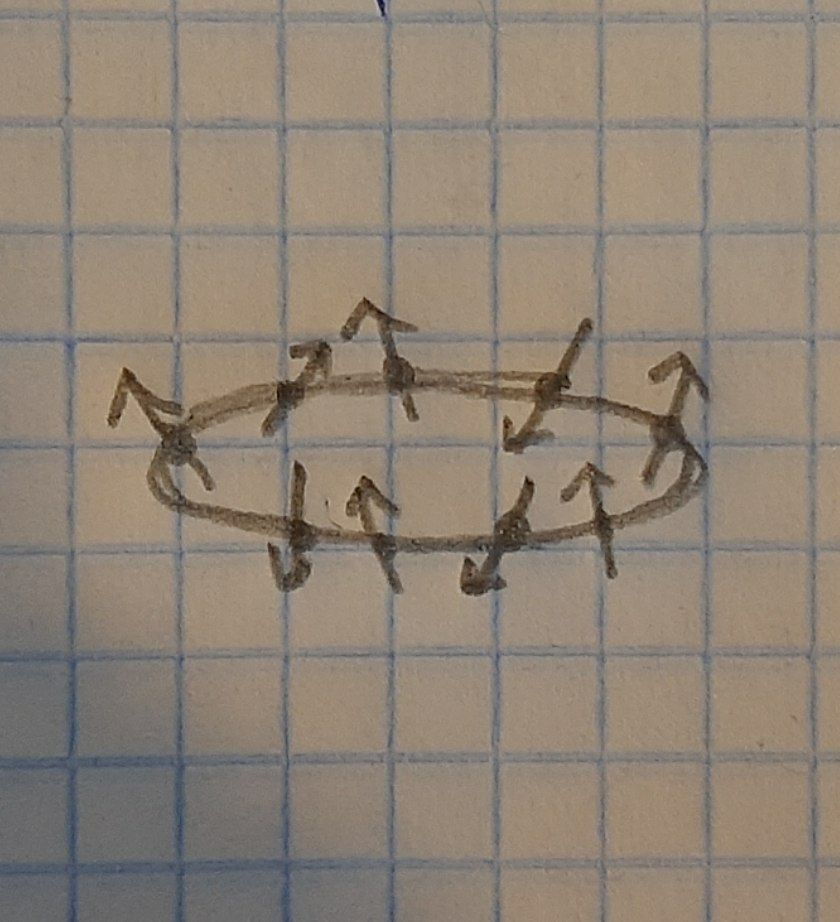
\includegraphics[width=0.5\linewidth]{chapter3/figures_special/isingchain1.jpg}
      \caption{Cadena de Ising abierta.}
    \end{subfigure}%
    \begin{subfigure}{0.5\textwidth}
      \centering
      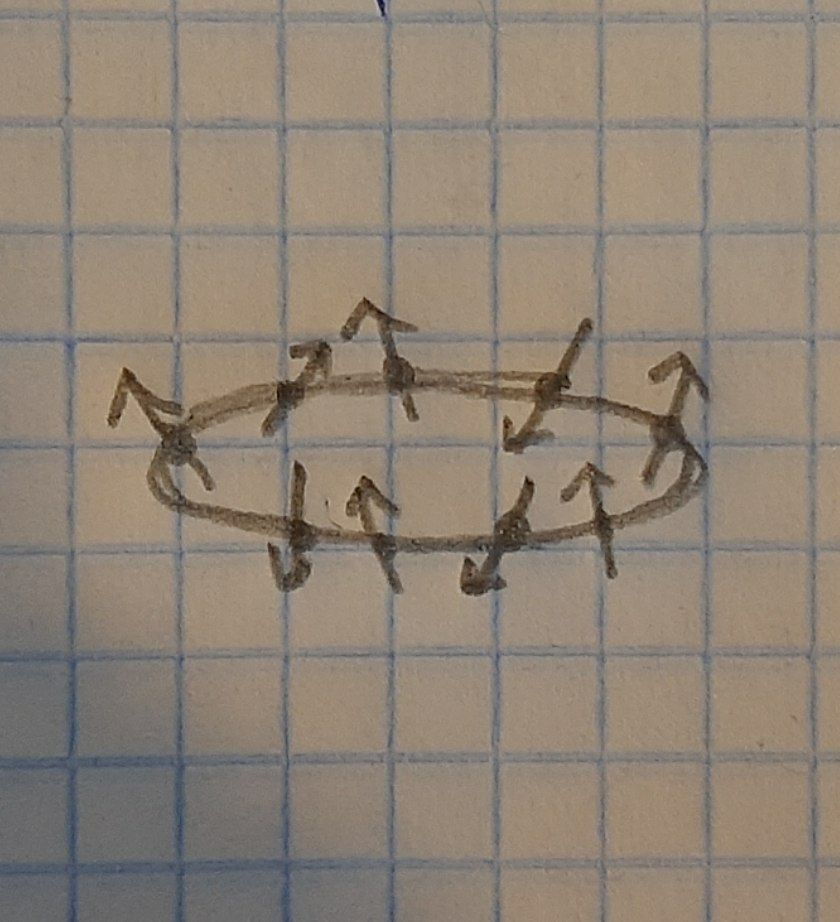
\includegraphics[width=0.5\linewidth]{chapter3/figures_special/isingchain1.jpg}
      \caption{Cadena de Ising cerrada}
    \end{subfigure}
    \label{fig:IsingChainOpenAndClosed}
\end{figure}
Sea entonces $\rho_{\ef}\in\densityspace{2}$ un estado efectivo correspondiente a un sistema de $n=2$ partículas, y $\varrho_{\max}$ el estado microscópico compatible con $\rho_{\ef}$ que maximiza la entropía. El hamiltoniano del sistema microscópico es, explícitamente,
\begin{equation}
    H=\omega\qty(\pauli{3}\otimes\pauli{3}),\nonumber
\end{equation}
de tal forma que dicho sistema evoluciona de acuerdo al operador unitario
\begin{equation}
    U=\Id \cos(\omega t)+ \rmi \pauli{3}\otimes\pauli{3} \sin(\omega t).\nonumber
\end{equation}
Si se propaga al estado de máxima entropía con dicho operador y se le pasa por la aplicación de grano grueso, la dinámica efectiva es
\begin{align}
    \Gamma_{t}(\rho_{\ef})=&\rho_{\ef} \cos^{2}(\omega)+\pauli{3} \rho_{\ef} \pauli{3} \sin^{2}(\omega t)\nonumber\\
    & + \rmi \sin(\omega t)\cos(\omega t)\qty(p_{1}\expval{\pauli{3}}_{2}[\pauli{3},\rho_{1}]+p_{2}\expval{\pauli{3}}_{1}[\pauli{3},\rho_{2}]).\nonumber
\end{align}
Dentro de la expresión de la dinámica efectiva reconocemos dos términos. El primero es un canal de desfasamiento sobre el estado efectivo, mientras que el segundo depende tanto de los parámetros de la aplicación de grano grueso, $p_{1}$ y $p_{2}$, como de valores esperados con respecto a los operadores de densidad reducidos del estado de máxima entropía. En efecto, el caso límite $p_{1}=1$ ve la dinámica efectiva reducida a un canal de desfasamiento en el tiempo,
\begin{equation}
    \Gamma_{t}(\rho_{\ef})=\rho_{\ef} \cos^{2}(\omega)+\pauli{3} \rho_{\ef} \pauli{3} \sin^{2}(\omega t).\nonumber
\end{equation}
mientras que el caso $p_{1}=p_{2}=\frac{1}{2}$ puede ser más informativo respecto al segundo término, pues en dicho caso
\begin{equation}
    \Gamma_{t}(\rho_{\ef})=\rho_{\ef} \cos^{2}(\omega)+\pauli{3} \rho_{\ef} \pauli{3} \sin^{2}(\omega t) + i\expval{\pauli{3}} \qty[\pauli{3},\rho_{\ef}] \sin(\omega t)\cos(\omega t).\nonumber
\end{equation}
Nótese que si $\expval{\pauli{3}}=1$, la dinámica es no solo lineal, sino unitaria, y corresponde a una rotación respecto al eje $z$, (con el detalle de que los estados tales que $\expval{\pauli{3}}=1$ son invariantes bajo dichas rotaciones). En realidad, el efecto de la dinámica efectiva sobre el estado es más clara en términos del vector de Bloch del estado inicial, $\vec{r}_{\ef}$.
\begin{equation}
    \Gamma_{t}(\vec{r}_{\ef})=\begin{pmatrix}
        x\cos(2\omega t)-yz\sin(2\omega t)\\
        xz\sin(2\omega t)+y\cos(2\omega t)\\
        z\\
    \end{pmatrix}.\nonumber
\end{equation}

La dinámica aplicada al vector de Bloch desplaza este en trayectoria elíptica centrada en el origen. A diferencia de una rotación circular, que tiene como único parámetro al ángulo de rotación, una rotación elíptica depende de los parámetros de la elipse, ambos semiejes y un argumento de rotación de la elipse, además del ángulo de rotación. En este caso, el vector de Bloch rota $2\omega t$ grados, a lo largo de la elipse de semieje mayor $\sqrt{1-z^2}$, semieje menor $z\sqrt{x^2+y^2}$ y argumento de rotación $\arccos(x)$. Esto es, los parámetros de la transformación dependen completamente del estado efectivo inicial. En este sentido, la dinámica es no lineal y no universal. La figura \ref{fig:Ising_p0.5_Sequence} presenta la evolución de la esfera de Bloch para el caso especial $p_{1}=\frac{1}{2}$.

\begin{figure}[ht!]
    \centering
    \begin{subfigure}{0.32\textwidth}
      \centering
      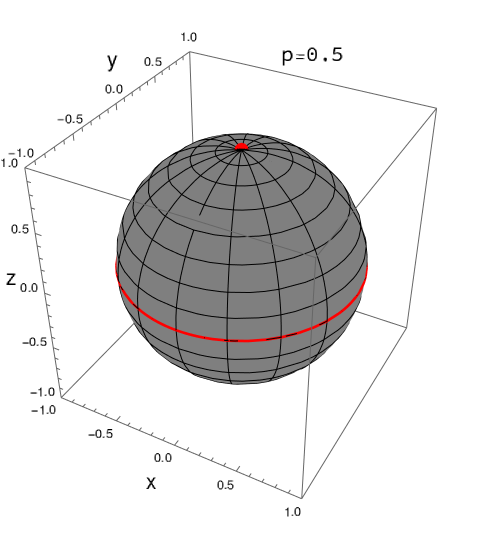
\includegraphics[width=0.9\linewidth]{chapter3/figures_special/sphere_Ising_t=0._z=0.9_p=0.5.png}
      \caption{$t=0$}
    \end{subfigure}%
    \begin{subfigure}{0.32\textwidth}
      \centering
      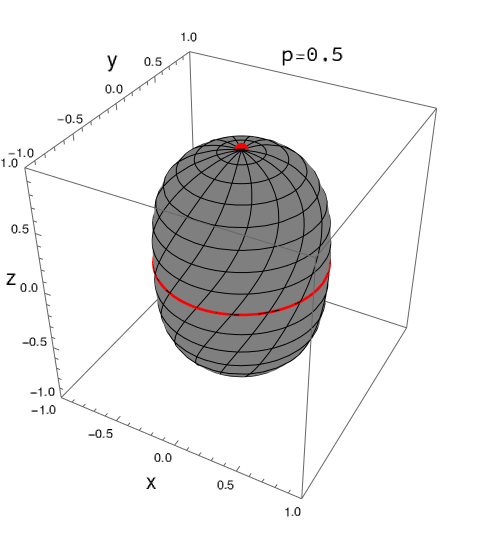
\includegraphics[width=0.9\linewidth]{chapter3/figures_special/sphere_Ising_t=0.5_z=0.9_p=0.5.png}
      \caption{$t=0.5$}
    \end{subfigure}
    \begin{subfigure}{0.32\textwidth}
      \centering
      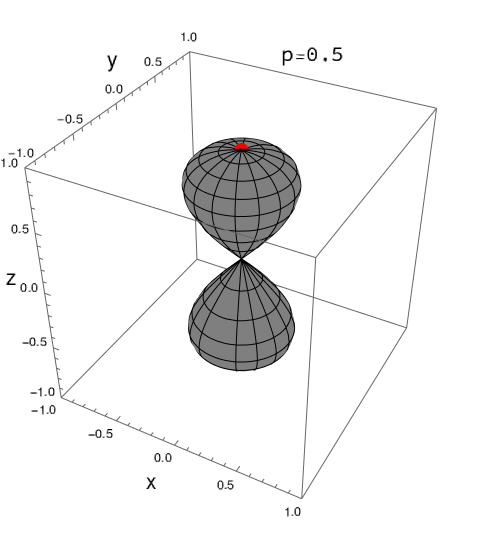
\includegraphics[width=0.9\linewidth]{chapter3/figures_special/sphere_Ising_t=1._z=0.9_p=0.5.png}
      \caption{$t=1$}
    \end{subfigure}
    \caption{Efecto del la evolución sobre la esfera de Bloch cuando $p=\frac{1}{2}$. Nótese que el desfasamiento sólo se completa en el eje $xy$.}
    \label{fig:Ising_p0.5_Sequence}
    \end{figure}

Como es natural, la expresión de la dinámica efectiva se vuelve cada vez más complicada y menos informativa conforme se aumenta el número de partículas. La dinámica unitaria general para la cadena de Ising cerrada sin campo transversal es
\begin{align}
    U=&\qty(\cos^{n}(\omega t)+(-\rmi)^{n}\sin^{n}(\omega t))\Id\nonumber\\ 
    &+\sum_{k=2}^{n-1}(-\rmi)^{n-k}\cos^{k}(\omega t)\sin^{n-k}(\omega t)\sum_{k_{1}<k_{2}}(\pauli{3,k_{1}}\pauli{3,k_{1}+1})(\pauli{3,k_{2}}\pauli{3,k_{2}+1}),\nonumber
\end{align}
mientras que para la cadena de Ising abierta es
\begin{align}
    U=&\cos^{n}(\omega t)\Id+(-\rmi)^{n}\sin^{n}(\omega t)\pauli{3,1}\pauli{3,n}\nonumber\\ 
    &+\sum_{k=2}^{n-1}(-\rmi)^{n-k}\cos^{k}(\omega t)\sin^{n-k}(\omega t)\sum_{k_{1}<k_{2}}(\pauli{3,k_{1}}\pauli{3,k_{1}+1})(\pauli{3,k_{2}}\pauli{3,k_{2}+1}).\nonumber
\end{align}
Si se quisiera hallar la dinámica efectiva, esta tendría términos dependientes de los valores esperados de todos los operadores $\pauli{3}^{\vec{j}}$ donde $\vec{j}$ tiene $n-1$ entradas, cosa que se traduce como un mínimo de $2^{n-1}$ términos. Aunque en este trabajo no se buscarán dichas expresiones, es posible usar calculadoras simbólicas para obtener visualizaciones de dichas dinámicas efectivas. Las figuras \ref{fig:Ising_n=3} a \ref{fig:Ising_n=8} muestran estas visualizaciones, mientras que las figuras \ref*{fig:Ising_n=3} a \ref{fig:Ising_n=8} muestran la trayectoria de diferentes vectores de Bloch efectivos bajo las mismas dinámicas.

\begin{figure}
    \centering
    \begin{subfigure}[b]{0.475\textwidth}
        \centering
        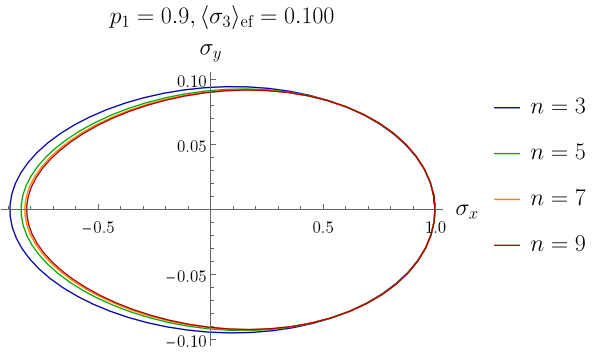
\includegraphics[width=\textwidth]{chapter3/figures_special/Ising_open_preferential_equal_p_n=n_r=1._z=0.10_p1=0.9.png}
        \caption{$p_{1}=0.9$}  
        \label{fig:OpenIsingPure1}
    \end{subfigure}
    \hfill
    \begin{subfigure}[b]{0.475\textwidth}  
        \centering 
        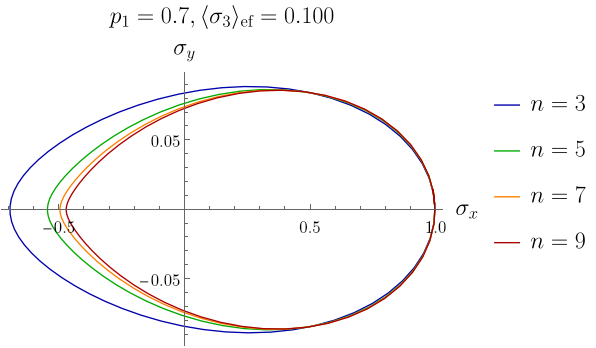
\includegraphics[width=\textwidth]{chapter3/figures_special/Ising_open_preferential_equal_p_n=n_r=1._z=0.10_p1=0.7.png}
        \caption{$p_{1}=0.7$}    
        \label{fig:OpenIsingPure2}
    \end{subfigure}
    \vskip\baselineskip
    \begin{subfigure}[b]{0.475\textwidth}   
        \centering 
        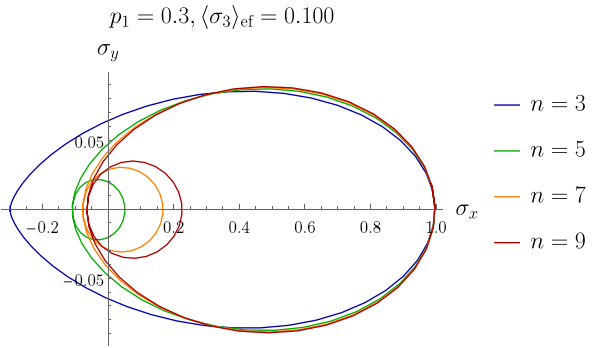
\includegraphics[width=\textwidth]{chapter3/figures_special/Ising_open_preferential_equal_p_n=n_r=1._z=0.10_p1=0.3.png}
        \caption{$p_{1}=0.3$}   
        \label{fig:OpenIsingPure3}
    \end{subfigure}
    \hfill
    \begin{subfigure}[b]{0.475\textwidth}   
        \centering 
        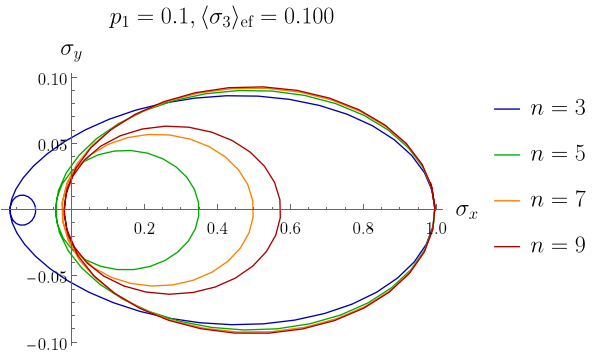
\includegraphics[width=\textwidth]{chapter3/figures_special/Ising_open_preferential_equal_p_n=n_r=1._z=0.10_p1=0.1.png}
        \caption{$p_{1}=0.1$}    
        \label{fig:OpenIsingPure4}
    \end{subfigure}
    \caption{Trayectorias del vector de Bloch de $\rho_{\ef}$ para si $r_{\ef}=1$ a una altura $z_{\ef}=0.1$, para diferentes valores de $n$ y $p_{1}$}
    \label{fig:OpenIsingPure}
\end{figure}

En general, los reusultados son no lineales. Se observa que, en los casos en los que se escoge $p_{k}=\frac{1}{n-1}\,\forall\,k\neq 1$, la evolución acerca más al estado efectivo hacia el desfasamiento. Para el caso en que las probabilidades diferentes a la de la primera partícula son aleatorias, los resultados son variados. El caso en que $p_{k}=\frac{1}{n-1}\,\forall\,k$. El caso en que el estado efectivo inicial es puro,
\acnote{hoy se me hizo algo tarde pero  tengo que obtener figuras como las que obtuve hoy para el caso puro y para el caso del Boltzman. Ya con eso se termina este capítulo.}

\acnote{agregar interpretación de los resultados numéricos}. Debido a que el tamaño de las matrices requeridas para el cálculo de la dinámica efectiva de un sistema microscópico de $n$ partículas aumenta como $2^{n}$, no fue posible obtener resultados numéricos para $n$ grande.



\newpage